%% This is an example first chapter.  You should put chapter/appendix that you
%% write into a separate file, and add a line \include{yourfilename} to
%% main.tex, where `yourfilename.tex' is the name of the chapter/appendix file.
%% You can process specific files by typing their names in at the 
%% \files=
%% prompt when you run the file main.tex through LaTeX.
\chapter{Introduction}
\label{chap:intro}

In the past few years, the development of \textit{Robotics} has surpassed people's expectation. The word \textit{Robotics} first appeared in the science fiction "Liar!" by Issac Asimov~\cite{wiki:Robotics}, and it referred to the science and technology of robots. By definition, \textit{Robotics} is a research branch that related to design, control and application of robots, as well as processing feedback from robots. 

Modern robots have been classified into several categories (\eg, mobile robot, industrial robot, service robot, education robot, \etc) according to their usages. Among these categories, full-autonomous and semi-autonomous mobile robot attracts special attentions. Such robots have the abilities to move around, with or without human control. The aim of the research in mobile robot is to help us accomplish various hard tasks, whether these tasks are performed domestically, commercially or militarily. These tasks, such as assisting disabled people, defusing bombs, and repairing equipment in dangerous places are either risky or high expense for human beings.    

For mobile robot, finding physical location of itself in the unknown environment is normally crucial, and such an ability (\textit{Robot Navigation}) allows mobile robot to avoid risky obstacles and finally arrive the goal position. Roughly speaking, Robot Navigation is a computing system which processes the information from external sources (\eg, sensors), applies an algorithm to navigate robot, and sometimes builds a map of the external environment. In Robot Navigation, robots sense environmental information by their sensors. These sensors, either locally (\eg, camera, inertial measurement unit (IMU)), or globally (\eg, global positioning system (GPS)) detect environmental changes, and eventually transfer their data to robots. Generally, sensors equipped in mobile robot (local sensor) are designed to be light-weighted, small, and inexpensive considering movement convenience and low expense. Among various types of local sensors, camera and IMU sensor are considered as the most common local sensors in small mobile robot system.

A camera is a optical instrument for image captures. Modern camera has several advantages for Robot Navigation. First, the core of camera chip-set is cheap and easily installed in any mobile robot platform; Second, camera often brings rich information as it simulates the functioning of human eye. By recognizing key-points ~\cite{shi1994good, lowe1999object, rosten2010faster} in certain images, system observes \textit{landmarks} in environment, and those landmarks will help to localize robots by \textit{Triangulation} ~\cite{davison2003real, klein2007parallel, eade2007monocular}.

An IMU sensor (Figure~\ref{fig:fig1-1}) usually consists of \textit{gyroscope}, \textit{accelerometer}, and sometimes \textit{magnetometer}, to measure specific force, angular rate and magnetic field regarding to its local frame. IMU is one of the major component in \textit{Inertial Navigation System}, which is firstly used in air plane, spacecraft, guided missiles, and now also in mobile robot ~\cite{batalin2004mobile, lee2009position, mourikis2007multi, forster2015imu}. IMU sensor utilizes \textit{Dead Reckoning} to track the position of devices. Dead Reckoning integrates IMU data over time by assuming the movement model of devices is fixed (\ie, acceleration and rotation rate is constant over a small period of time). 

\begin{figure}
    \centering
    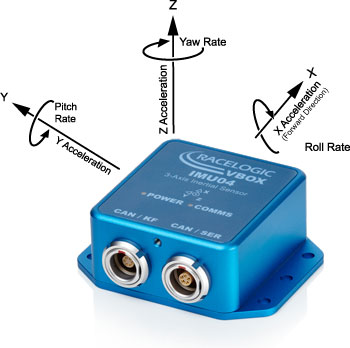
\includegraphics[width=0.5\textwidth]{CONTENT/Figure/Figure1-1_IMU_Sensor.jpg}
    \caption{IMU sensor with gyroscope and accelerometer measures rotational rate and acceleration of X, Y, and Z axis regarding its local frame. Note that IMU sensor normally has bias and irreducible noises, and it is necessary to apply a calibration similar to the camera calibrations. The frequency of IMU output is normally larger than 100 [Hz]. Source: \cite{Figure1-1_IMU_Sensor}}
    \label{fig:fig1-1}
\end{figure}


\section{Motivation and Contribution}
\label{sec:motiv_contrib}

The main motivation of this thesis is to improve the navigation accuracy by fusing camera data and IMU sensor data. 

Single sensor-based navigation system may not fully satisfy the requirements of high-quality localization. GPS-based navigation system has been used for outdoor devices for a long time. However, such a system suffered from localizing in \textbf{in-door} environment, and also the accuracy of general GPS is not sufficient, it usually has error from 3 to 5 meters \cite{wiki:GPS}. However, for a mobile robot, which may move from in-door to out-door, GPS is mostly not used, and the performance of GPS is usually served as the baseline of navigation~\cite{hesch2014consistency}.   

Vision-based navigation system \cite{davison2003real, klein2007parallel}, or simultaneous localization and mapping (SLAM)~\cite{davison2007monoslam, engel2014lsd, mur2015orb} gives an acceptable navigation result for mobile robot. In \cite{davison2003real}, they recognize corner features to form the landmarks, and it uses an extended Kalman filter framework to track the uncertainty and propagates the system state, however it can not handle large-scale scene since the number of visual features will directly affect the computational time. \cite{klein2007parallel} utilizes key-frame based bundle adjustment to update the map, which improves both accuracy and efficiency, though it will have some issues in large-scale scene since vision-based method often leads to a trade-off between computational complexity and localization accuracy due to the rich information and low output frequency by camera. \cite{mur2015orb} is another application of keyframe-based SLAM, however it can not handle the situation with fast-moving cameras.

Single Inertial Navigation System recognizes target pose by \textit{Dead Reckoning}~\cite{mcnaughton1991dead, levi1996dead}. The problem of Dead Reckoning is error accumulation; only few directions are observable~\cite{hesch2014consistency} by IMU whole navigation process. When the object corrupt movement assumption, a correction step is often required.

Fusing camera data and IMU data has many advantages. On the one hand, high-frequency IMU data is an adequate compensation to low-frequency camera data; on the other hand, it is convenient to correct IMU integration by vision-based navigation results. Fusing camera data and IMU data for robot navigation is not novel. \cite{mourikis2007multi} applies multi-state Kalman filter (MSCKF) to update system states, which decreases the computational complexity by only storing last few keyframes. \cite{hesch2014consistency} discusses the inconsistency of MSCKF, and it provides a more accurate approach to propagate system states, therefore it increases the accuracy and robustness. \cite{forster2015imu} exploits a tightly-coupled way to optimize VIO problems on manifold by including image features and IMU measurements in cost function, and it increases the efficiency by eliminating support variables \cite{carlone2014eliminating} in their factor graph. 

The contributions of this thesis are as follows,
\begin{itemize}
\item {We exploit a highly flexible, realistic tool to generate synthetic IMU sensor data and corresponding image sequences, which have provided experimental data in this thesis.}
\item {We present the error-state Kalman filter system kinematic based on quaternion, we also explore multiple ways to integrate IMU data regarding to the different movement models.}
\item {We propose a novel approach, key-framed bundle adjustment, to augment fusing results}
\item {We propose a real-time visual-inertial framework implemented in C\texttt{++}, we demonstrate several experiments to show it is stable, scalable, high-accuracy and low-latency.}
\end{itemize}

\section{Outline of the Thesis}
\label{sec:outline}

In Chapter \ref{chap:Overview} we first introduce the world representations and useful notations in our visual-inertial odometry. We also compare the filter method and keyframe-based method in visual SLAM problem, and in the end we explain why we choose keyframe-based method in our loosely-coupled IMU integration framework.

Chapter \ref{chap:background} discusses \textit{Quaternion Algebra}. In this chapter, we introduce the basic operations on quaternion, the relationship among quaternions, rotation matrices and rotation vectors. Followed by that, we explain how to integrate or differentiate quaternion over time, which are the major tools to propagate quaternions.

Chapter \ref{chap:sensor_fusing} is the main part of this thesis. In Section \ref{sec:ESKF_IMU}, we study the error-state Kalman filter (ESKF), which is applied to IMU integration. Section \ref{sec:camera_comple_data} summarizes the approaches to fuse visual SLAM results into ESKF, including the adapted map scale method and keyframe-based bundle adjustment. In Section \ref{sec:pipeline_summary}, we overview the pipeline of our visual-inertial odometry system.

Experiment results are shown in Chapter \ref{chap:experiments}. First, the process of generating synthetic IMU and camera data is presented. Then we demonstrate several experiments to show that our proposed real-time visual-inertial odometry has higher accuracy and stability than the single IMU integration or visual SLAM when dealing with same data sequences. We evaluate the break-up timings of our system at last.

We briefly introduce our current researches in Chapter \ref{chap:current}. We suggest a way to form a cost function in order to solve our visual-inertial odometry via nonlinear optimization in Section \ref{sec:map}, then a standard way of manifold optimization is presented in Section \ref{sec:exponential}.

At last, we summarize and discuss our current works and potential future works in Chapter \ref{chap:summary}.
